\documentclass{article}
\usepackage[margin=0.8in]{geometry}
\usepackage{tikz}
\begin{document}
\section*{Disjoint enrollment preparation}
Preparation only: one native plan-only invocation and retained-slot verification. No empirical solves or new cost result. Clock qualification, scientific admission, budgets and analysis/export integration remain pending.\par
The retained seven original plans are partitioned into eight enrolled plans: p739 gate (60 workloads), cohort16 remainder (120), and six unchanged plans (180 each). Complete workload objects, methods and exact integer slot identities were checked by native preparation. Sequence and workload-array positions may differ and remain recorded in the mappings.\par
\begin{center}\begin{tabular}{lr}Workloads & 1,260\\Planned slots & 22,680\\Measured arm slots & 18,900\\Warmup slots & 3,780\\Measured candidate/reference pairs & 6,300\\Empirical solver executions & 0\end{tabular}\end{center}
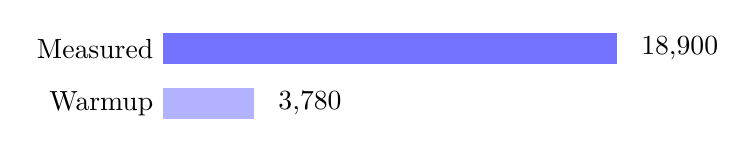
\begin{tikzpicture}[x=0.0003cm,y=1cm]
\node[anchor=east] at (0,0) {Measured};\fill[blue!55] (0,-0.2) rectangle (18900,0.2);\node[anchor=west] at (19500,0) {18,900};
\node[anchor=east] at (0,-0.7) {Warmup};\fill[blue!30] (0,-0.9) rectangle (3780,-0.5);\node[anchor=west] at (4400,-0.7) {3,780};
\end{tikzpicture}
\subsection*{Evidence and limits}
The request and native outputs are retained byte-for-byte. The certificate and mappings preserve both original and enrolled identities. The separate upper gate is not included in this partition. Earlier p739 observations and their invalid clock status are not changed. This packet contains no cost estimate and authorizes no execution.\par
Source receipt SHA-256:\par\texttt{\small b33c6acb87806e63104f7f1b0bcc1ecbb5f2f5760a9cc1026b5819a864eff4e9}\par
Machine-readable observations: report.json. Graph: enrollment.svg. Raw evidence and software-test receipts are bound by the packet manifest.
\end{document}
